\documentclass[paper=a4, fontsize=11pt]{scrartcl} % A4 paper and 11pt font size
\usepackage{listings} 
\usepackage[T1]{fontenc} % Use 8-bit encoding that has 256 glyphs
\usepackage{fourier} % Use the Adobe Utopia font for the document - comment this line to return to the LaTeX default
\usepackage[english]{babel} % English language/hyphenation
\usepackage{amsmath,amsfonts,amsthm} % Math packages
\usepackage{graphicx}
\usepackage{lipsum} % Used for inserting dummy 'Lorem ipsum' text into the template
\usepackage{amsmath,amsfonts}
\usepackage{sectsty} % Allows customizing section commands
\allsectionsfont{\centering \normalfont\scshape} % Make all sections centered, the default font and small caps
\usepackage{MnSymbol}
\usepackage{paralist}
\usepackage{float}
\usepackage{fancyhdr} % Custom headers and footers
\pagestyle{fancyplain} % Makes all pages in the document conform to the custom headers and footers
\fancyhead{} % No page header - if you want one, create it in the same way as the footers below
\fancyfoot[L]{} % Empty left footer
\fancyfoot[C]{} % Empty center footer
\fancyfoot[R]{\thepage} % Page numbering for right footer
\renewcommand{\headrulewidth}{0pt} % Remove header underlines
\renewcommand{\footrulewidth}{0pt} % Remove footer underlines
\setlength{\headheight}{13.6pt} % Customize the height of the header
\usepackage[labelformat=empty]{caption}
\numberwithin{equation}{section} % Number equations within sections (i.e. 1.1, 1.2, 2.1, 2.2 instead of 1, 2, 3, 4)
\numberwithin{figure}{section} % Number figures within sections (i.e. 1.1, 1.2, 2.1, 2.2 instead of 1, 2, 3, 4)
\numberwithin{table}{section} % Number tables within sections (i.e. 1.1, 1.2, 2.1, 2.2 instead of 1, 2, 3, 4)

\setlength\parindent{0pt} % Removes all indentation from paragraphs - comment this line for an assignment with lots of text
\usepackage{amsmath}
\usepackage{mathtools}
\lstset{
	mathescape,
	escapeinside={(*@}{@*)}
}
%----------------------------------------------------------------------------------------
%	TITLE SECTION
%----------------------------------------------------------------------------------------

%\begin{lstlisting}
%write code here
%\end{lstlisting}

%math mode: $

%\end{itemize}
%\begin{figure}[h]
%  \centering
%  \includegraphics[width=0.55\textwidth]{img/image}
%  \caption{caption}
%  \label{fig:boat1}
%\end{figure}


\newcommand{\horrule}[1]{\rule{\linewidth}{#1}} % Create horizontal rule command with 1 argument of height

\title{	
\normalfont \normalsize 
\textsc{Ca' Foscari University of Venice, MSc Computer Science, Cybersecurity} \\ [25pt] % Your university, school and/or department name(s)
\horrule{0.5pt} \\[0.4cm] % Thin top horizontal rule
\huge Advanced Algorithms and Programming Methods: Distributed Algorithms \\ % The assignment title
\horrule{2pt} \\[0.5cm] % Thick bottom horizontal rule
}

\begin{document}

\maketitle % Print the title

\section*{Broadcast: the FLOODING algorithm}
\textbf{Definition} \\
Consider a distributed computing system where only one entity $x$ knows some important information; this entity would like to share this knowledge with all the other entities in the system. This problem is called \textit{broadcasting}.

Solving this problem means designing a set of rules that, when executed by the entities, will lead to a configuration in which all entities know the information; the solution must work regardless of which entity has the information at the beginning.

According to this, broadcasting requires connectivity restrictions to be solved: in particular, every entity has to be reachable from every other entity. \\ \\

\textbf{Time and Message complexity} \\
We will denote by $M(Bcast)$ and $T(Bcast)$ the message and time complexity.

The first message is sent by the initiator and has to reach all the entities.

Given $d(a, b)$ the distance, i.e., the minimal number of edges between $a$ and $b$, the ideal time depends on the time spent to go from the initiator to any node, thus the \textit{eccentricity} or radius of G.
$$r(initiator) = Max\{d(x,y) : x,y \in V\}$$
~ \\
Given that any node can be the initiator, we need to compute the diameter of the graph:
$$T(Bcast) = diameter(G) \leq n-1 = \mathcal{O}(n)$$
We consider $m$ as the number of links. We could say that there will be $\leq$ 2 messages on each link.

Let $s$ be our initiator: 
\begin{align*}
	M(Bcast) &= |N(s)| + \sum_{x \neq s} (|N(x)|-1) 
			 = \sum_{x}|N(x)| - \sum_{x \neq s}1 
	         = 2m - (n-1)
\end{align*}

The \textit{flooding} algorithm has optimal time complexity, but the number of messages sent can be reduced! In fact, $M(BCast) \ge m = \Omega(m)$ and $M(Flooding) = 2m - n + 1$. 

~ \\

\textbf{Assumptions}\\ 
Before proceeding with the actual code, we need to make some assumptions about the solution we are providing. In particular:
\begin{compactitem}
	\item Unique initiator: the initiator is unique by definition of the problem
	\item Total reliability \& bidirectional link: to simplify the solution
	\item G is connected: otherwise the problem would be unsolvable for a given initiator K
\end{compactitem}
~\\
\textbf{Code} 
\\ We have to consider three different states -INITIATOR, SLEEPING, DONE- and two possible events -spontaneous impulse event and receiving of a message.

\begin{lstlisting}
if INITIATOR
	(*@\textit{spontaneous impulse event}@*)
		send(I) to N(X)
		become (DONE)
	(*@\textit{receiving(I)}@*)
		do-nothing
if SLEEPING
	(*@\textit{receiving(I)}@*)
		send(I) to N(x) - {sender}
		become(DONE)
	(*@\textit{spontaneous impulse event}@*)
		do-nothing
if DONE
	(*@\textit{receiving(I)}@*)
		do-nothing
	(*@\textit{spontaneous impulse event}@*)
		do-nothing				
\end{lstlisting}

Notice that if the system is asynchronous, many different executions are possible, depending on the speed at which messages travel.

It is also worth noting that in a distributed environment the entities end their computations at different points in time, hence there is only a concept of \textit{local termination} instead of a \textit{global} one. No entity knows when the entire process terminates!


\section*{Protocol SHOUT}
We are assuming that there is a single initiator, there are bidirectional links, there is total reliability and G is connected. \\ \\
\textbf{Preliminary: definition of Spanning Tree} \\ 
A spanning tree T of a graph G = (V, E) is an acyclic subgraph of G such that T' = (V, E') and\\ E' $\subseteq$ E.
\\ ~ \\
\textbf{Definition} \\
We want to build a spanning tree in a distributed system, but we have to consider that the entities do not know G, not even its size. The only things an entity is aware of are the labels on the ports leading to its neighbors and the fact that, if it sends a message to a neighbor, the message will eventually be received.\\~\\
\textbf{Solution} ~ ~ \textit{Ask-Your-Neighbors}
\begin{compactitem}
\item The initiator $s$ will send a message Q = ('Are you my neighbor in the spanning tree?') to all its neighbors
\item An entity $x \neq s$ will reply 'Yes' only the first time it is asked and, in this occasion, it will ask all its other neighbors; otherwise it will reply 'No'.
\item Each entity terminates when it has received a reply from all neighbors to which it asked the question.
\end{compactitem}
\begin{figure}[H]
  \centering
  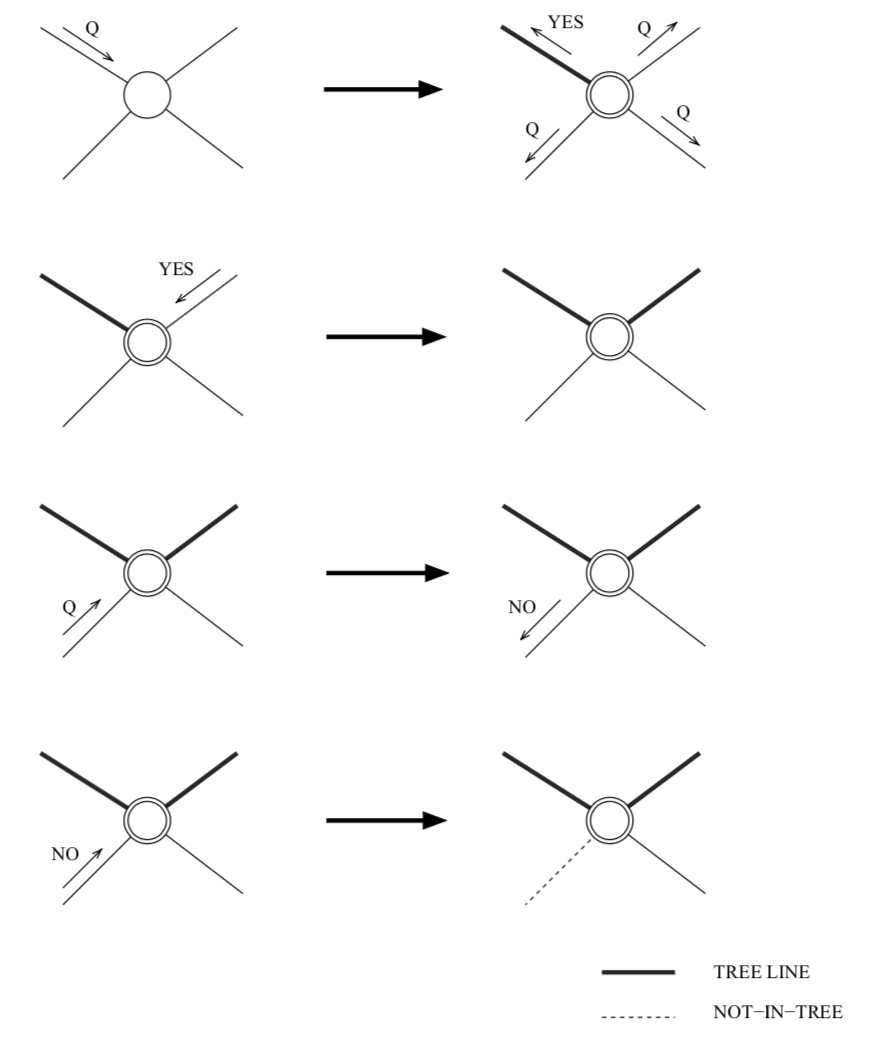
\includegraphics[width=0.9\textwidth]{img/shout.png}
  \caption{Example of SHOUT}
  \label{fig:boat1}
\end{figure}
\newpage
\textbf{Code:} We have four states, INITIATOR, IDLE, ACTIVE, DONE; the terminal state is DONE.
\begin{lstlisting}
if INITIATOR
	(*@\textit{spontaneous impulse event}@*)
		root = true
		tree-neighbors = {}
		send(Q) to N(x)
		counter = 0
		become ACTIVE
if IDLE
	(*@\textit{receiving(Q)}@*)
		root = false
		parent = sender
		tree-neighbors = {sender}
		send('Yes') to sender
		counter = 1
		//managing leaves and intermediate node cases
		if counter = |N(x)| then
			become DONE
		else
			send (Q) to N(x) - {sender}
			become ACTIVE			 
if ACTIVE
	(*@\textit{receiving(Q)}@*)
		send ('No') to sender
	(*@\textit{receiving('Yes')}@*)
		tree-neighbors = tree-neighbors $\cup$ sender
		counter += 1
		if counter = |N(x)|
			become DONE
	(*@\textit{receiving('No')}@*)
		counter += 1
		if counter = |N(x)|
			become DONE			
\end{lstlisting}
\textbf{Complexity} \\
First of all, notice that \textit{shout} can be assimilated to a combination of \textit{flood} and \textit{reply}. In other words, $M(SHOUT) = 2	\times M(FLOOD)$.
To compute the total amount of messages sent in this protocol we have to consider the messages sent by the initiator, plus the other messages Q sent, plus the amount of 'Yes' and 'No' answers.
\begin{align*}
	M(SHOUT) &= Q + NO  + YES \\ 
	&= (n-1)+ 2\times(m-(n-1)) + 2\times(m-(n-1)) + (n-1) \\
	&= 4m - 2n + 2 = 2\times(2m-n+1)
\end{align*}

\subsection*{SHOUT+}
We might wonder that SHOUT could be improved. For example, we might avoid sending all the 'No' messages.
\\ This is the idea behind the SHOUT+ algorithm. In fact, the code is almost the same as SHOUT, but we do not need to send the 'No' message. Of course, this change needs to be managed.\\
In order to do this, we only need to change the ACTIVE state.
\begin{lstlisting}
if ACTIVE
	(*@\textit{receiving(Q)}@*)
		send ('No') to sender
	(*@\textit{receiving('Yes')}@*)
		tree-neighbors = tree-neighbors $\cup$ sender
		counter += 1
		if counter = |N(x)|
			become DONE
	(*@\textit{receiving('No')}@*)
		counter += 1
		if counter = |N(x)|
			become DONE	
\end{lstlisting}
is replaced by 
\begin{lstlisting}
if ACTIVE
	(*@\textit{receiving(Q)}@*)
		counter += 1
		if counter = |N(x)|
			become(DONE)
	(*@\textit{receiving('Yes')}@*)
		tree-neighbors = tree-neighbors $\cup$ sender
		counter += 1
		if counter = |N(x)|
			become DONE
\end{lstlisting}
\textbf{Complexity} \\
The messages are much less. 
$M(SHOUT+) = 2m$ while $M(SHOUT) = 2(2m -n+1)$

\clearpage
\section*{Leader election}
\textbf{Definition} \\
Moving the system from an initial configuration where all entities are in the same state (called \textit{available}), into a final configuration where all entities are in the same state (called \textit{follower}), except one which is in a different state (called \textit{leader}).\\
We assume a bidirectional graph, connected and no failures.\\

\subsection*{Saturation technique}
This technique is used to solve many other problems, independently from the number and positions of the initiators (there might be multiple initiators).\\
The states are \textit{available}, \textit{awake} and \textit{processing}. The algorithm can be divided in three parts:
\begin{compactitem}
\item Activation phase: started by all initiators, consists in a ``wake-up" -  all nodes are \textit{activated}
\item Saturation phase: started by the leaves, a unique pair of neighbors is identified (\textit{saturated nodes}), the other become \textit{processing}.
\item Resolution phase: started by the saturated nodes, it varies depending on the protocol
\end{compactitem}~\\
\textbf{Code} \\ We have four states AVAILABLE, ACTIVE, PROCESSING, SATURATED. The initial state is AVAILABLE.
\begin{lstlisting}
if AVAILABLE (*@ ~ ~ \textit{I haven't been activated yet}@*)
	(*@\textit{spontaneously}@*)
		send('Activate') to N(x)
		neighbors = N(x)
		if |neighbors| = 1 (*@ ~ ~ \textit{leaf case}@*)
			parent = neighbors
			send('Saturation') to parent
			become(PROCESSING)
		else
			become(ACTIVE)	
	(*@\textit{receiving('Activate')}@*)
		send('Activate') to N(x) - {sender}
		neighbors = N(x)
		if |neighbors| = 1
			parent = neighbors
			send('Saturation') to parent
			become(PROCESSING)
		else
			become(ACTIVE)


if ACTIVE
	(*@\textit{receiving(M)}@*)
	neighbors = neighbors - {sender}
	if |neighbors| = 1
		parent = neighbors
		send('Saturation') to parent
		become(PROCESSING)

if PROCESSING
	(*@\textit{receiving(M)}@*)
		become(SATURATED)					
\end{lstlisting}


\textbf{Complexity} 
$$M(Saturation) = 2n -2+n+n-2 = 4(n-1)$$ 
But how can this technique be useful for our election problem?
~ \\

\subsection*{Solution to the election problem}
Let us assume we assign a label $v(x)$ to each node (notice that if nodes are indistinguishable, ranking is unsolvable). Then, it is possible to:
\begin{compactenum}
\item Run the saturation technique
\item The two saturated nodes exchange the value and if it is different they can elect as a leader the one with smaller value.\\
Observations:
\begin{compactitem}
	\item If nodes do not have distinct labels, the leader cannot be elected.
	\item Each saturated node knows where the other one is, since it knows from which edge it has received the last message.
\end{compactitem}
\end{compactenum}

\clearpage 
\subsection*{Minimum finding with saturation technique}
Each entity $x$ has in input its value $value(x)$. At the end each entity should know whether it is the minimum or not.\\

\textbf{Code} \\
The states are AVAILABLE, ACTIVE, PROCESSING, MINIMUM, LARGE. The starting state is AVAILABLE.
\begin{lstlisting}
if AVAILABLE
	(*@\textit{spontaneously}@*)
		send('Activate') to N(x)
		min = v(x)
		neighbors = N(x)
		if |neigbours| = 1 //leaf
			M = ('Saturation', min)
			parent = neighbors
			send(M) to parent
			become(PROCESSING)
		else
			become(ACTIVE)
	(*@\textit{receiving('Activate')}@*)
		send('Activate') to N(x) - {sender}
		min = v(x)
		neighbors = N(x)
		if |neighbors| = 1	//leaf
			M = ('Saturation', min)
			parent = neighbors
			send(M) to parent
			become(PROCESSING)
		else
			become(ACTIVE)
if ACTIVE
	(*@\textit{receiving(M)}@*)
		min = min{min, M}
		neighbors = neighbors - {sender}
		if |neighbors| = 1 //leaf
			M = ('Saturation', min)
			parent = neighbors	
			send(M) to parent
			become(PROCESSING)
\end{lstlisting}
\newpage
\begin{lstlisting}			
if PROCESSING
	(*@\textit{receiving(M)}@*)
		min = MIN{min, M}
		notification = ('Resolution', min)
		send (Notification) to N(X) - parent
		if v(x) = min
			become MINIMUM
		else
			become LARGE									
\end{lstlisting}
\textbf{Complexity} \\
$M(minimum) = 2\times(n-1) + n + n - 2$ where $2\times(n-1)$ is the cost for the activation; $n$ the cost for saturation and $n - 2$ the cost for notification.$M(minimum) = 4n - 4 = \mathcal{O}(n)$
\\ ~ \\
\subsection*{Ranking problem in arbitrary networks}
\textbf{Definition:} \\Given a graph G(V, E) rank it from the lowest value to the largest.\\ ~ \\
\textbf{Solution}\\In an arbitrary network, this problem could be solved in the following way:
\begin{compactitem}
\item Find a spanning tree
\item Use saturation and the minimum finding to find a starting node
\item Do ranking (Centralized or De-centralized)
\end{compactitem}
\subsubsection*{Centralized ranking}
This problem could be solved in the following way:
\begin{compactitem}
\item Build a spanning tree using SHOUT algorithm
\item Elect a leader (minimum) using saturation technique
\item The leader knows the minimum, it sends in that direction a ranking message.
\item Every node knows the minimum in its subtrees, it can then forward the ranking message (ranking, minimum) in the right direction.
\item When the node to be ranked receives the message it sends up a notification and update message \textit{(new-minimum)} that will travel up to the leader.
\end{compactitem}
~ \\
\textbf{Complexity}
$$M(rank\_centr) = 2\times(n-1)+ 2\times(n-2)+ ... + 2(1)= n\times(n-1)$$ 
\clearpage
\subsubsection*{De-centralized ranking}
\textbf{Solution}\\
The starter node sends a ranking message of the form \textit{(first, second, rank)} in the direction of the first. The first has the smallest value, the second the second smallest known so far. If no value is indicated (or the value is $\infty$ ) it means that the smallest in the corresponding subtree is unknown (at the moment).\\
The ranked node attempts to send a ranking message to the next node to be ranked. The second variable of the rank message is updated during its travel and the minimum values on the links of the tree are also updated.\\ ~ \\
\textbf{Complexity} \\ $M(rank\_decentr) = 2\times(n-1)+ (n-2)+ (n-3)+ ...+ 1= (n-1)n/2+ (n-1)= (n-1)(\frac{n}{2}+1)$ \\ ~ \\
\textbf{Code}
\begin{compactitem}
\item Build a spanning tree using SHOUT
\item We elect a leader (e.i. minimum using saturation technique)
\item Jump from the min to the second one and so on using messages of the form\\ \textit{(first, second, \#rank)}. After having elected the minimum, we know the second smallest element and so we send a message with \textit{(secondValue, $\infty$ , 2nd)}: this message travels across the spanning tree to find the third element. After the second receives the message, set the value of the subtree as $\infty$ because there is nothing to rank in that subtree - and so on. 
\end{compactitem}
~ \\ 
\subsection*{Election problem}
The election problem cannot be generally solved if the entities do not have different identities.\\
Consider a synchronous system where the entities are unique, have the same state and are anonymous.
At each moment, they are doing the same thing, receive the same messages, move to the same states.\\ In such a system, it is impossible to elect a leader, because the entities are indistinguishable. That is why we need entities with different identities.\\
Notice that with distinct IDs, minimum finding is an election.
\\ ~ \\
\textbf{Election in trees}\\
To each node x is associated a distinct identifier v(x). \\ A simple algorithm:
\begin{compactitem}
\item Execute the saturation technique
\item Choose the saturated node holding the minimum value
\end{compactitem} ~ \\ 
\textbf{Election in rings}\\
A ring is a sparse network (few arcs) such as trees, but it's not symmetric. Every entity has two neighbors.
\clearpage
\subsubsection*{All The Way}
Each ID is fully circulated in the ring, hence each entity sees all identities.
\\
Assumptions:
\begin{compactitem}
\item Two versions: unidirectional and bidirectional
\item Local orientation
\item Distinct identities
\end{compactitem}
All the entities can be the initiators. The bidirectional version assumes that the ring is oriented. The protocol works even without knowing the dimension of the ring and having messages that arrive in a non-FIFO order. \\ 
Ideally: each node sends it value; if it receives a message, it forwards it and it keeps track of the minimum value seen so far.\\ \\
\textbf{Code}\\The states are ASLEEP, AWAKE, FOLLOWER, LEADER; the starting state is ASLEEP and the terminal states are FOLLOWER and LEADER. 
\begin{lstlisting}
(*@\textit{// notice that INITIALIZE and CHECK are "macros" / functions}@*)
INITIALIZE
	count = 0
	size = 1
	known = false
	send('Election', id(x), size) to right
	min = id(x)

CHECK
	if count = ringsize
		if min = id(x)
			become(LEADER)
		else
			become(FOLLOWER)										

if ASLEEP
	(*@\textit{spontaneously}@*)
		INITIALIZE
		become(AWAKE)
	(*@\textit{receiving('Election', value, counter)}@*)
		INITIALIZE
		send('Election', value, counter+1) to other
		min = min{min, value}
		count = count + 1
		become(AWAKE)



if AWAKE
	(*@\textit{receiving('Election', value, counter)}@*)
		if value $\neq$ id(x)
			send('Election', value, counter+1) to other
			min = min{min, value}
			count+=1
			if known 
				CHECK
		else
			ringsize = counter
			known = true
			CHECK
\end{lstlisting}
\textbf{Complexity}\\
Each entity crosses each link, so the complexity is $\mathcal{O}(n)^2$; the size of each message is $log(id)$.\\
$M(Alltheway) =\mathcal{O}(n)^2$ messages \\
$T(Alltheway) \leq 2n-1 = \mathcal{O}(n)$ \\ \\
Observations:
\begin{compactitem}
\item The algorithm also solves the data collection problem
\item It works for both unidirectional and bidirectional cases
\end{compactitem}
\\ ~ \\ 
\subsubsection*{Another solution: AsFar (as it can)}
\textbf{Idea} \\ It is not necessary to send and receive messages with larger IDs than the IDs the current node has already seen.\\
Assumptions:
\begin{compactitem}
\item Unidirectional/bidirectional ring
\item Different id's
\item Local oriented
\end{compactitem}
\begin{figure}[H]
  \centering
  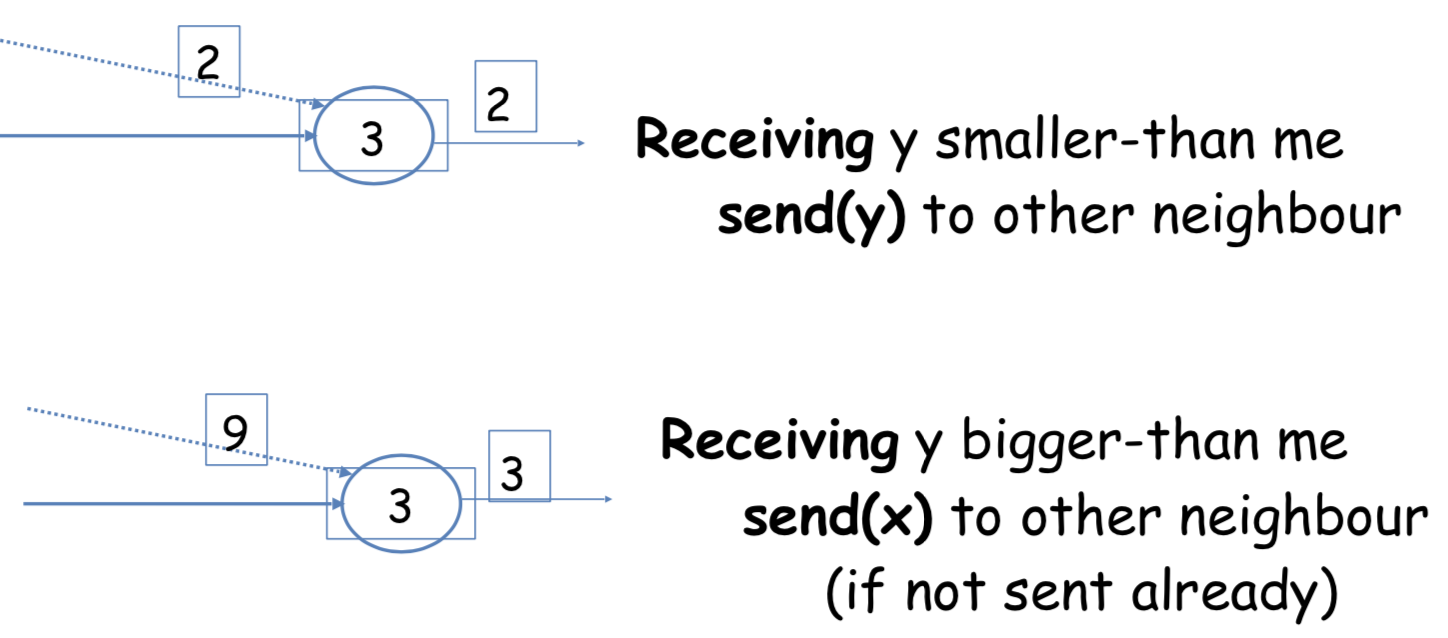
\includegraphics[width=0.9\textwidth]{img/asfar.png}
  \caption{AsFar example}
  \label{fig:boat1}
\end{figure}
\textbf{Code:} The states are ASLEEP, AWAKE, FOLLOWER, LEADER; the starting state is ASLEEP, the terminal states are FOLLOWER and LEADER.\\
\textbf{Unidirectional version:}
\begin{lstlisting}
if ASLEEP
	spontaneously
		send('Election', id(x)) to right
		min = id(x)
		become(AWAKE)
	receiving('Election', value)
		send('Election', id(x)) to right
		min = id(x)
		if value < min
			send('Election', value) to right
			min = value
		become(AWAKE)		
if AWAKE
	receiving('Election', value)
		if value < min
			send('Election', value) to right
			min = value
		else
			if value = min
				NOTIFY
	receiving(NOTIFY)
		send(NOTIFY) to other
		become(FOLLOWER)
NOTIFY
	send(NOTIFY) to right
	become(LEADER)						
\end{lstlisting}
\section*{Synchronous systems}
We consider as synchronous system all systems in which all local clocks are incremented by one unit symultaneously; in other words all local clocks 'tick' in the same moment. Notice that this assumption does not mean that all the clocks have the same value, but just that their values are incremented at the same time.\\ 
The first part of this section is about calculating how much time will take a message to be send in a synchronous system. (not going to treat this part)
\subsection*{Man-finding and election}
\textbf{General idea:} messages travel at different speed.
\begin{itemize}
\item Knowledge of n is not necessary
\item Unidirectional version
\item Synchronous
\end{itemize}
There are two ways of eliminating ids, one is like in AsFar, large ids are stopped by smaller ids; the other is that small ids travel faster so to catch up with larger ids and eliminate them. \\
\textbf{Important:} Each message travels at a speed which depends on the identity it contains.\\ 
Speed is assumed to be unitary, the same for every message. How can we change it? Introducing appropriate delays.\\
When a node receives a message containing i, it waits f(i) ticks. When a node receives its own id, it becomes the leader and sends a notification message around the ring. This message will not be delayed.\\
Another example could be done with f(i) = 2$^i$. When a node recives a message containing i, it waits 2$^i$ ticks. 
\begin{figure}[H]
  \centering
  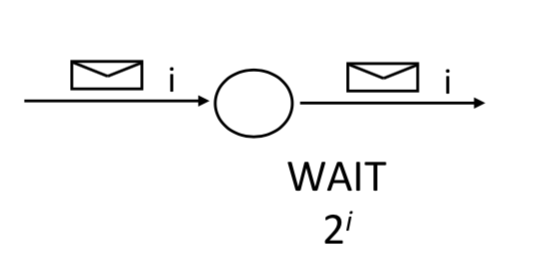
\includegraphics[width=0.4\textwidth]{img/fi.png}
  \caption{Graphical example of 2$^i$ delay}
  \label{fig:boat1}
\end{figure}
When a node receives its own id, it becomes the leader and sends a notification message around the ring. This message will not be delayed.\\
In time 2$^i$n + n the smallest id i traverses the ring. Let the second smallest be i+1 (waiting time 2$^{i+1}$). How many links does it have the time to traverse while the smallest id goes around? $$(2^i + n)/ 2^{i+1} \approx n/2$$
We can generalize that by thinking about the j$^{th}$ id: in time: $2^in + n$, has traversed $(n/2^j)$ links.
While: $$totalMessages = \sum_{j = 1}^{n-1} = n\sum_{j = 1}^{n-1}1/2^j=O(n)$$ 
So we can say that the total time is:$$totalComplexity = O(2^in)$$

\section*{Peer-to-peer}
\subsection*{Architecture}
\begin{figure}[H]
  \centering
  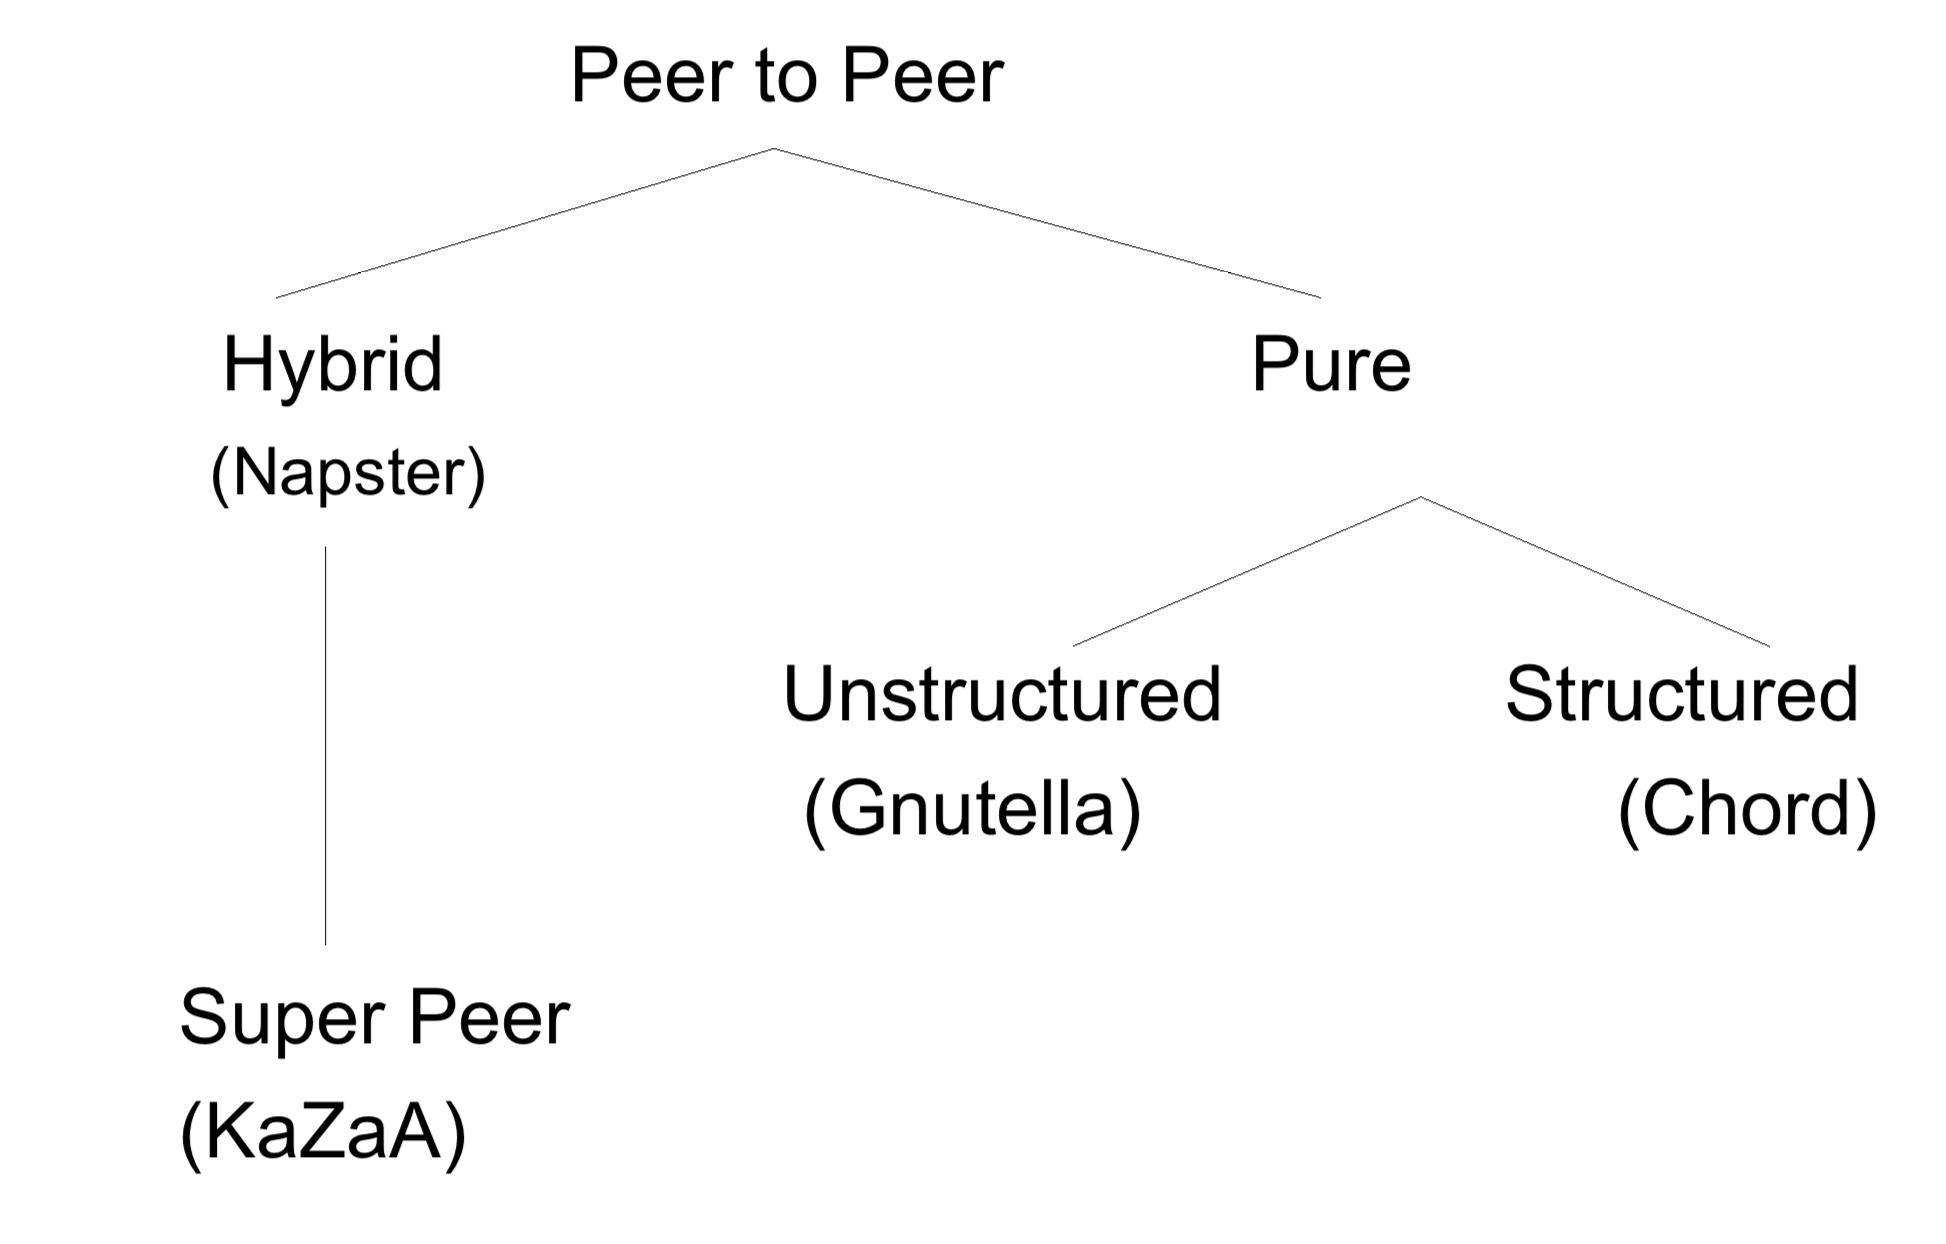
\includegraphics[width=0.6\textwidth]{img/p2p.png}
  \caption{p2p architecture}
  \label{fig:boat1}
\end{figure}

\subsection*{Search}
\subsubsection*{Hybrid p2p}
\textbf{Napster} presents a centralized lookup. The peers send metadata to the look-up server.\\
When a resource request arrives, the server returns the list of the peers that store the resource. Data are then exchanged among peers.
 \begin{figure}[H]
  \centering
  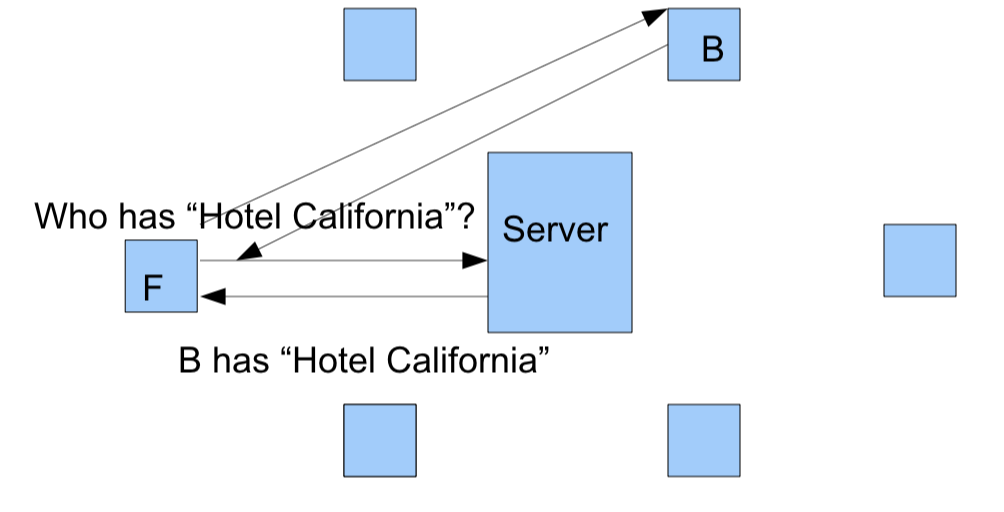
\includegraphics[width=0.6\textwidth]{img/search_n.png}
  \caption{Search in hybrid p2p systems}
  \label{fig:boat1}
\end{figure}
\subsubsection*{Unstructured pure p2p}
\textbf{Gnutella} is a pure p2p without a central server. Peers have an initial set of addresses known for the first connection; peers are equally treated, no metter which bandwidth they have and how many files they share. Each peer provides both the files and sends/replies to routing requests. Each peer is both client and server.\\
Each peer knows a subset of neighbouring peers, there are some cache servers that maintains as many peer addresses as possible; when the application starts, it contacts one of these cache servers that will add the p2p network to the new peer.\\
When the search starts, requests from a peer R are sent from neighbour to neighbour (PING). The message stops either when the resource is found or after a limited and predefined number of steps(TTL = time to live). If the resource has been found, the address of the peer P that stores it, sends to R(PONG). R will directly contact P and will download the resource.
\textbf{Problem:} hard to control/regulate 
 \begin{figure}[H]
  \centering
  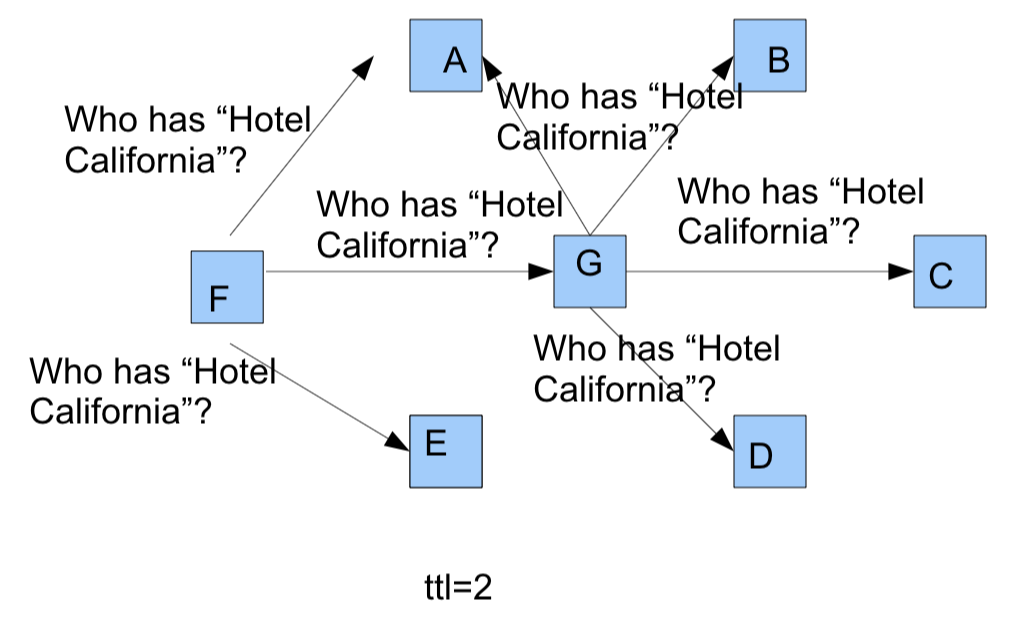
\includegraphics[width=0.55\textwidth]{img/gnu1.png}
  \caption{PING with Gnutella}
  \label{fig:boat1}
\end{figure}
 \begin{figure}[H]
  \centering
  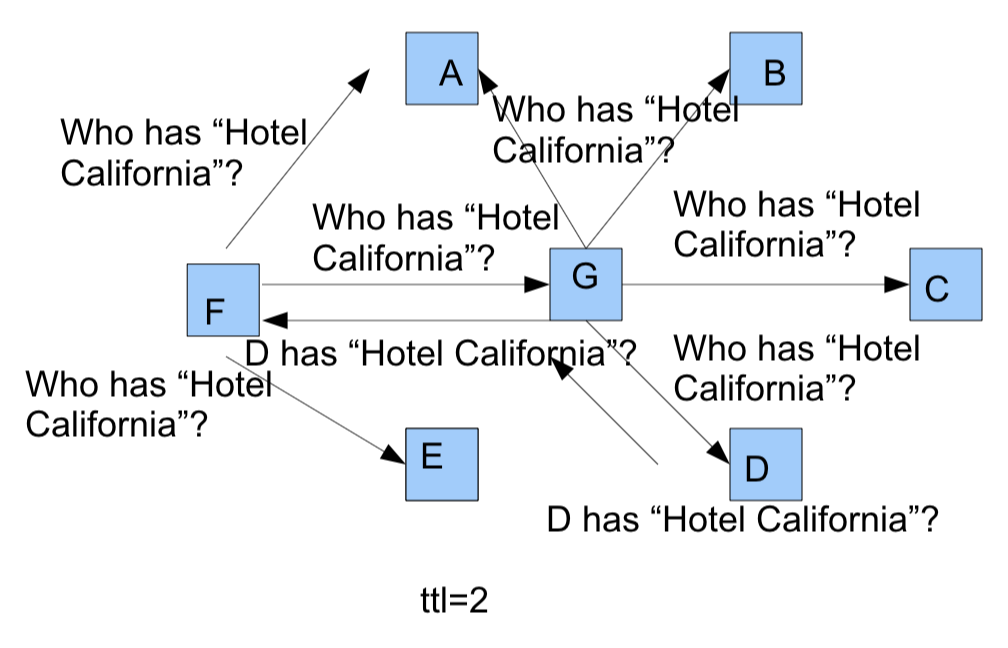
\includegraphics[width=0.55\textwidth]{img/gnu2.png}
  \caption{PONG with nutella}
  \label{fig:boat1}
\end{figure}
\subsubsection*{Iterative deepening}
\begin{itemize}
\item The system is flooded with a limited TTL
\item If the resource is not found, we start with a bigger TTL
\item We repeat up to when the resource is found or when a boundary TTL is found
Many variations: blind, informed...
\end{itemize}
\newpage
\subsubsection*{Super peer (ZaZaA)}
It behaves like a pure and a hybrid p2p system.
\begin{itemize}
\item There are different servers, the super peers supervives the subnetworks (subtrees)
\item The super peers execute the queries for the leaves (e.i. they work as servers)
\item The super peers are also operate as normal peers
\item The peers exchange information directly
\item Combine the characteristics of hybrid and pure systems
\end{itemize}
\textbf{Search?} We have to do some questions:
\begin{itemize}
\item Good numbers  of leaves for each super peer?
\item How should super peers connect together?
\item The system is made more reliable k redundant
\end{itemize}
\subsection*{Bit Torrent}
Many users can simultaneously download the same file without delay too much each other. Files are not downloaded from the same server but they are divided into different portions. Each peer that makes a request, offers already downloaded portions to the other peers, thus contributing to the downloading of the other peers.\\
We concentrate on the efficient fetching and not on the search. There is a single publisher and many downloaders. The same file is distributed among many peers. 
\subsection*{Information storage}
The main questions are: where to store information in a p2p system? How to find it?\\
Parameters: 
\begin{itemize}
\item System scalability: limit the communication overhead and the memory used by the nodes with respect to the number of nodes in the system.
\item Robustness and adaptability: in the presence of failures and changes
\end{itemize}
There could be many approach in which we can store our inforation.
\begin{itemize}
\item Centralized approach: we send a request to the server. We use $O(N)$ memory on the server, search $O(1)$ step to reach the server
\item Decentralized approach: we send a request to all our neighbors (different optimizations, e.i. TTL). We use $O(1)$ memory and we use $O(n^2)$ steps for the search.
\end{itemize}
Another approach is to have \textbf{distributed hash tables} in the system. It's a good compromise for what regard the complexity of the operations. We use $O(\log(N))$ steps to find the informations and $O(\log(N))$ entries in the routing table of each node.\\
Technique: 
\begin{itemize}
\item Adaptability: it is simple to insert (assing thge information) and remove nodes (reassignment to the neighbouring nodes)
\item Balances information on the nodes (makes routing efficient)
\end{itemize}
Peers and data are mapped in the same address space throungh hash functions. For nodes the hash of the IP; for data hash of the content (title, ...)\\
\subsection*{Chord}
\textbf{Data distribution:} data are distributed among peers using a precise algorithm. Data are replicated to improve availability.\\
\textbf{Assignment:}
\begin{itemize}
\item Each peer has an ID (hash of the IP)
\item Each resource has a key (hash of the title, ...)
\item We use long keys to avoid collision
\item The peers stores resources with keys similar to one of the peers
\item Given a key of a resource the peer sends the request to the peer with the most similar key
\end{itemize}
Using Chrod we have to use a consistent hashing:
\begin{itemize}
\item To assign the keys to the peers
\item There should be load balancing so that with very high probability each peer receives the same number of resources/keys
\item We ask for key updates when a peer connects/disconnects from the network
\item The insertion of the N-th key with hight probability will require the movement of 1/N other keys
\end{itemize}
\textbf{Advantages:}
\begin{itemize}
\item We maintain consisting hashing although the information is not stored in all the nodes
\item The system is simple, correctness and performance are easy to prove
\item It takes at most $O(\log(N))$ to reach the destination
\item A peer requires a table of $O(\log(N))$ bits for an efficent routing, but the performance decrease when the tables are not updated
\item The insertion/removal of a node generates $O(\log^2(N))$ messages
\end{itemize}
\textbf{Idea:} The logical space is circular O,..., 2$^m$-1, ring (mod 2$^m$). A resource with key K is stored in the node which is the closest successor from K (successor(K)).
 \begin{figure}[H]
  \centering
  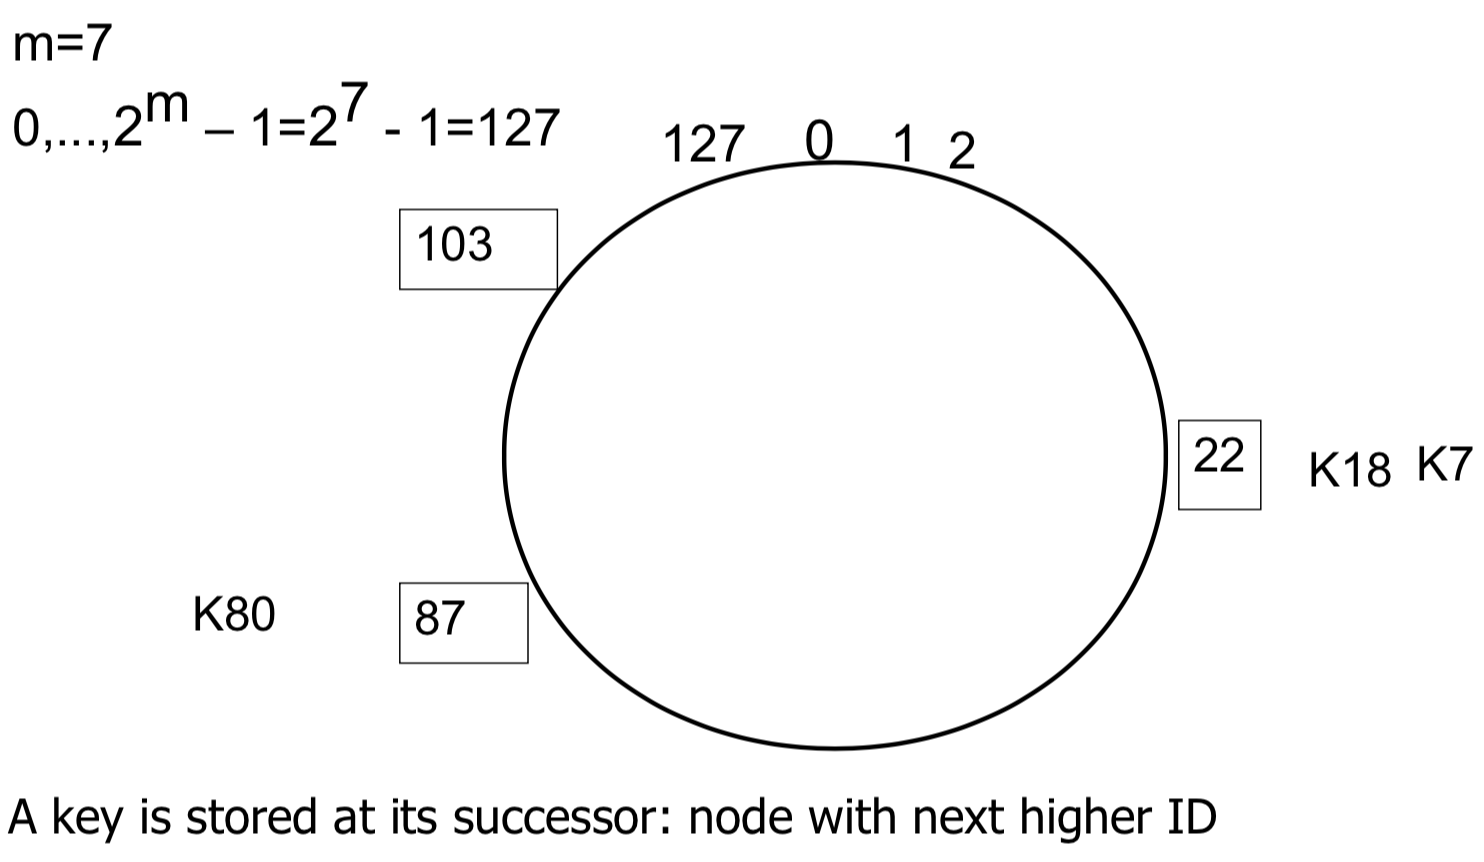
\includegraphics[width=0.6\textwidth]{img/chord_ex.png}
  \caption{Example of how Chord assign ID}
  \label{fig:boat1}
\end{figure}
\textbf{Successor:} the successor of peer 22 is 87, of 87 is 103, of 103 is 22.\\
\textbf{Routing:} each node stores only its successor. If the resource is not on this node, then the query is sent to the successor.\\
It requires $O(1)$ of memory, $O(N)$ for search: in the worst case we have to visit the whole ring. The failure of a node blocks the procedure.\\
This algorithm in the worst case it requires too many operations (we maintain other routing informations).\\
Note that this extra information is not required for the correctness of the procedure but it helps speeding up the search. This protocol works given that the calue of the next successor is correctly maintained/updated.\\
The best solution is that each node stores m values. The search of k is sent to the furthest known predecessor of k. We store more values of the close nodes and less of more distant nodes, routing is more precise close to a node. It requires $O(\log(N))$ of memory and $O(\log(N))$ for the search.\\
\textbf{Finger table}\\
Each node maintains a finger table (the i-th entry of the finger table of x is the first node that succeeds equals (x + 2$^i$) mod 2$^m$) and the predecessor node. An item is identified by id is stored on the successor node of id.
\subsubsection*{Examples}
Here below it will be provided some examples of how this algorithm works. 
 \begin{figure}[H]
  \centering
  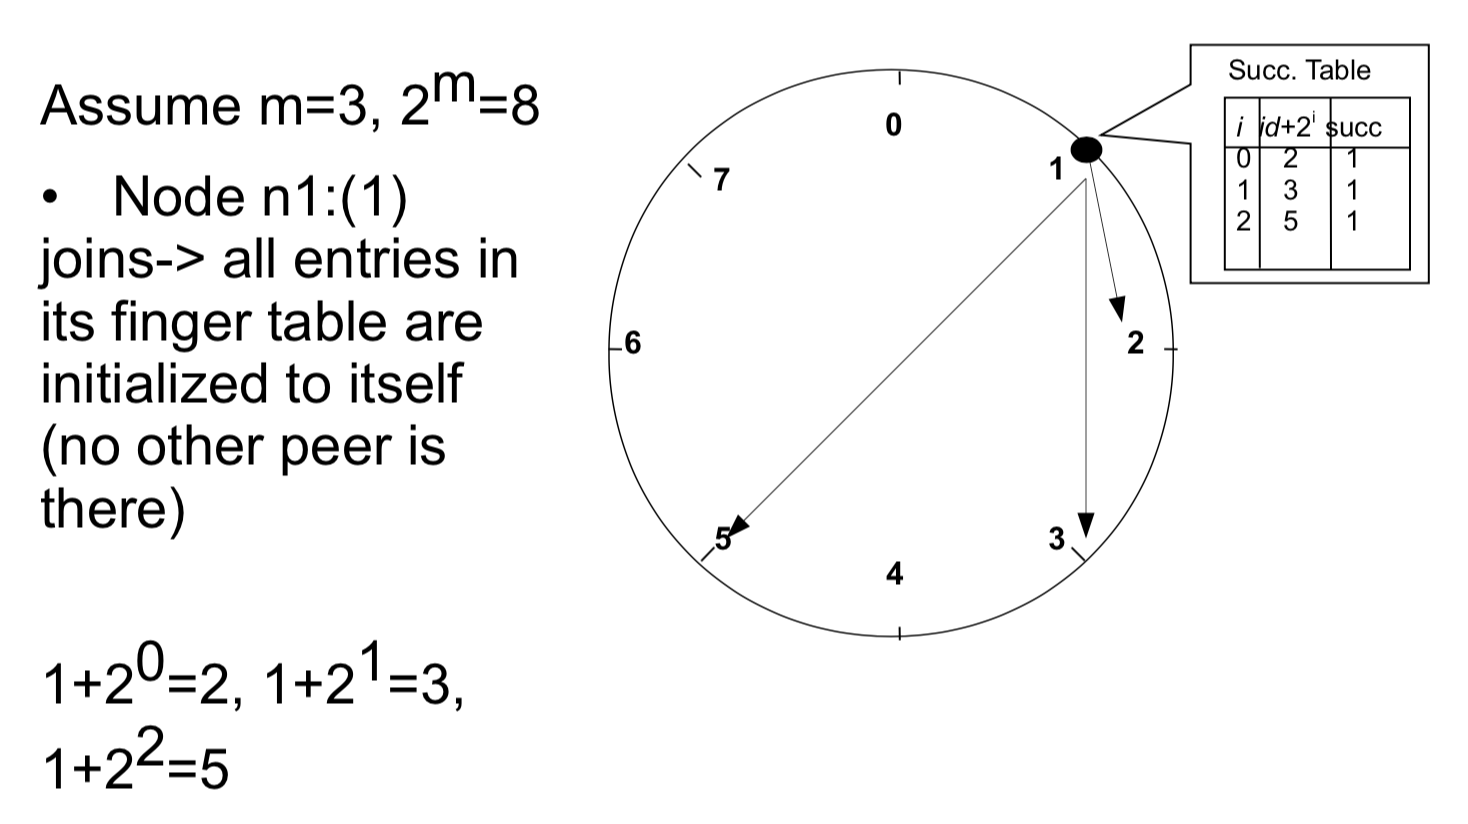
\includegraphics[width=1\textwidth]{img/chord1.png}
  \caption{First assignment with Chord}
  \label{fig:boat1}
\end{figure} \begin{figure}[H]
  \centering
  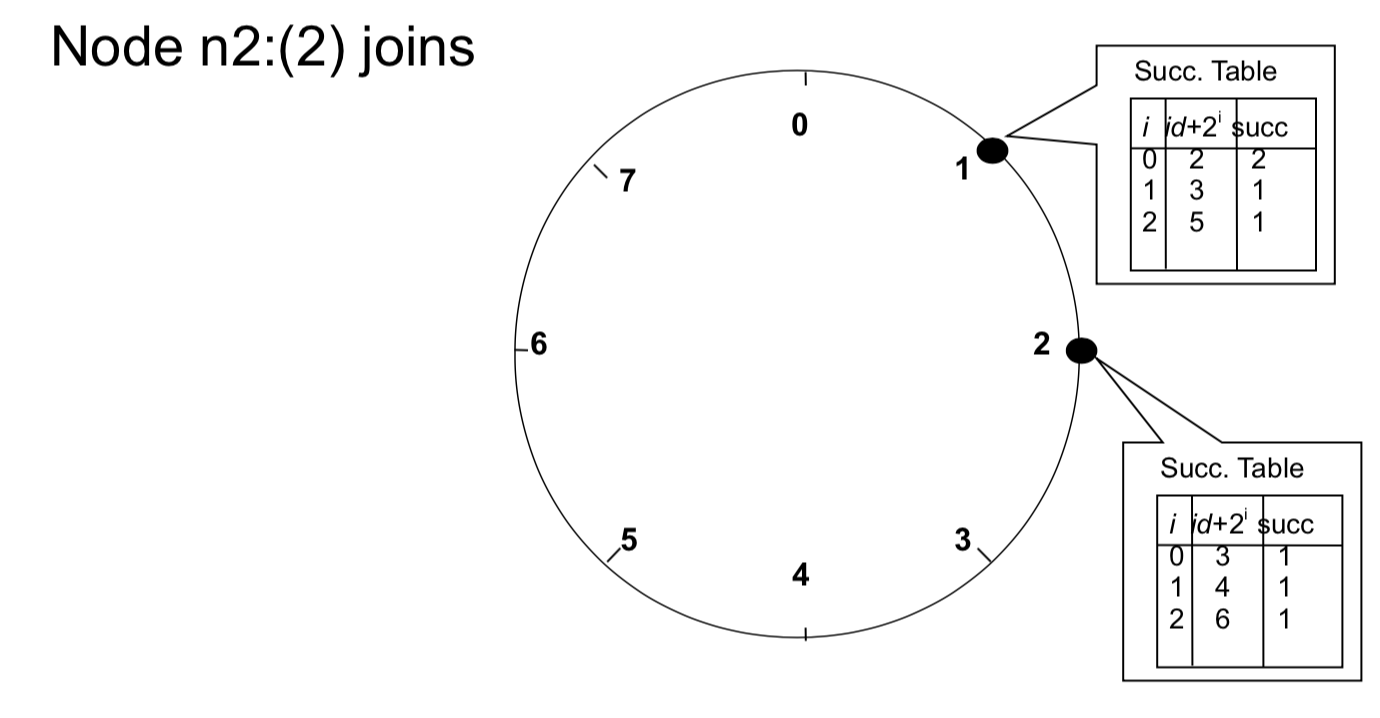
\includegraphics[width=1\textwidth]{img/chord2.png}
  \caption{Second node joins}
  \label{fig:boat1}
\end{figure} \begin{figure}[H]
  \centering
  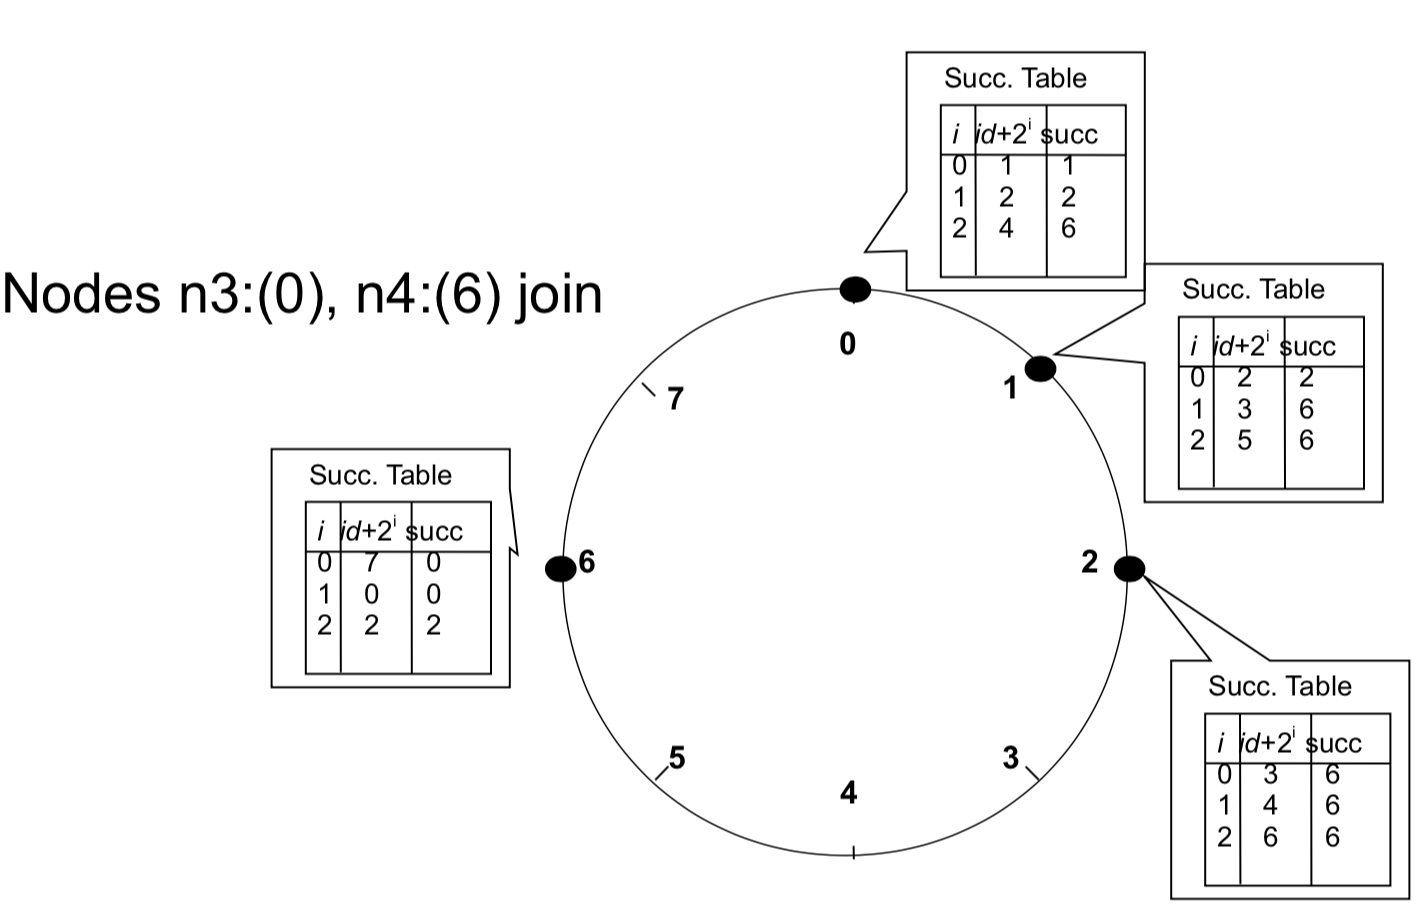
\includegraphics[width=1\textwidth]{img/chord3.png}
  \caption{Third and forth joins}
  \label{fig:boat1}
\end{figure}
 \begin{figure}[H]
  \centering
  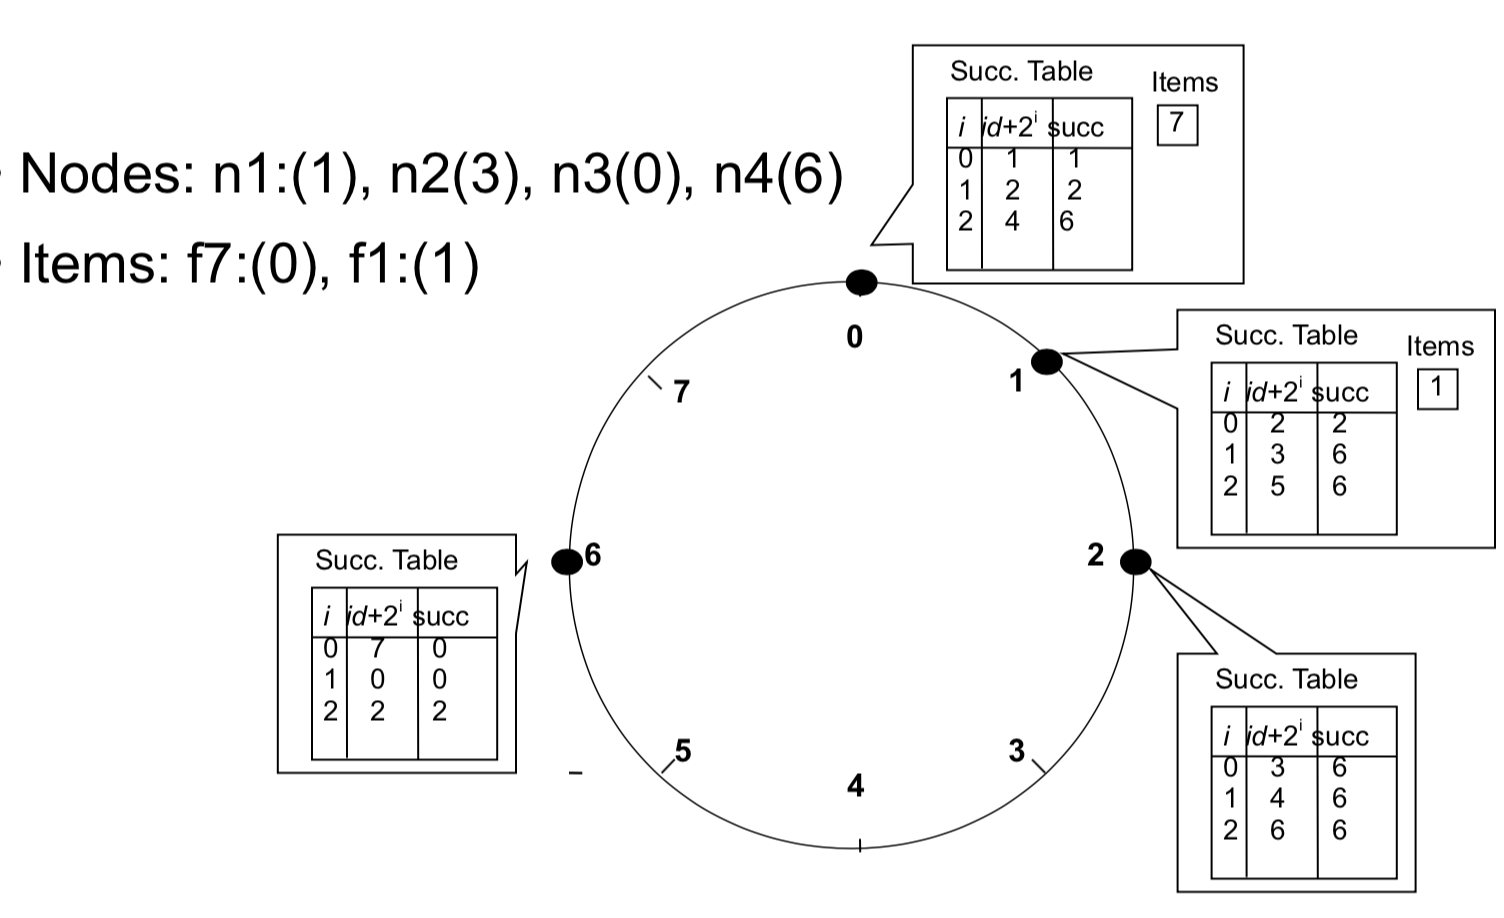
\includegraphics[width=1\textwidth]{img/chord4.png}
  \caption{Item assignment}
  \label{fig:boat1}
\end{figure}
 \begin{figure}[H]
  \centering
  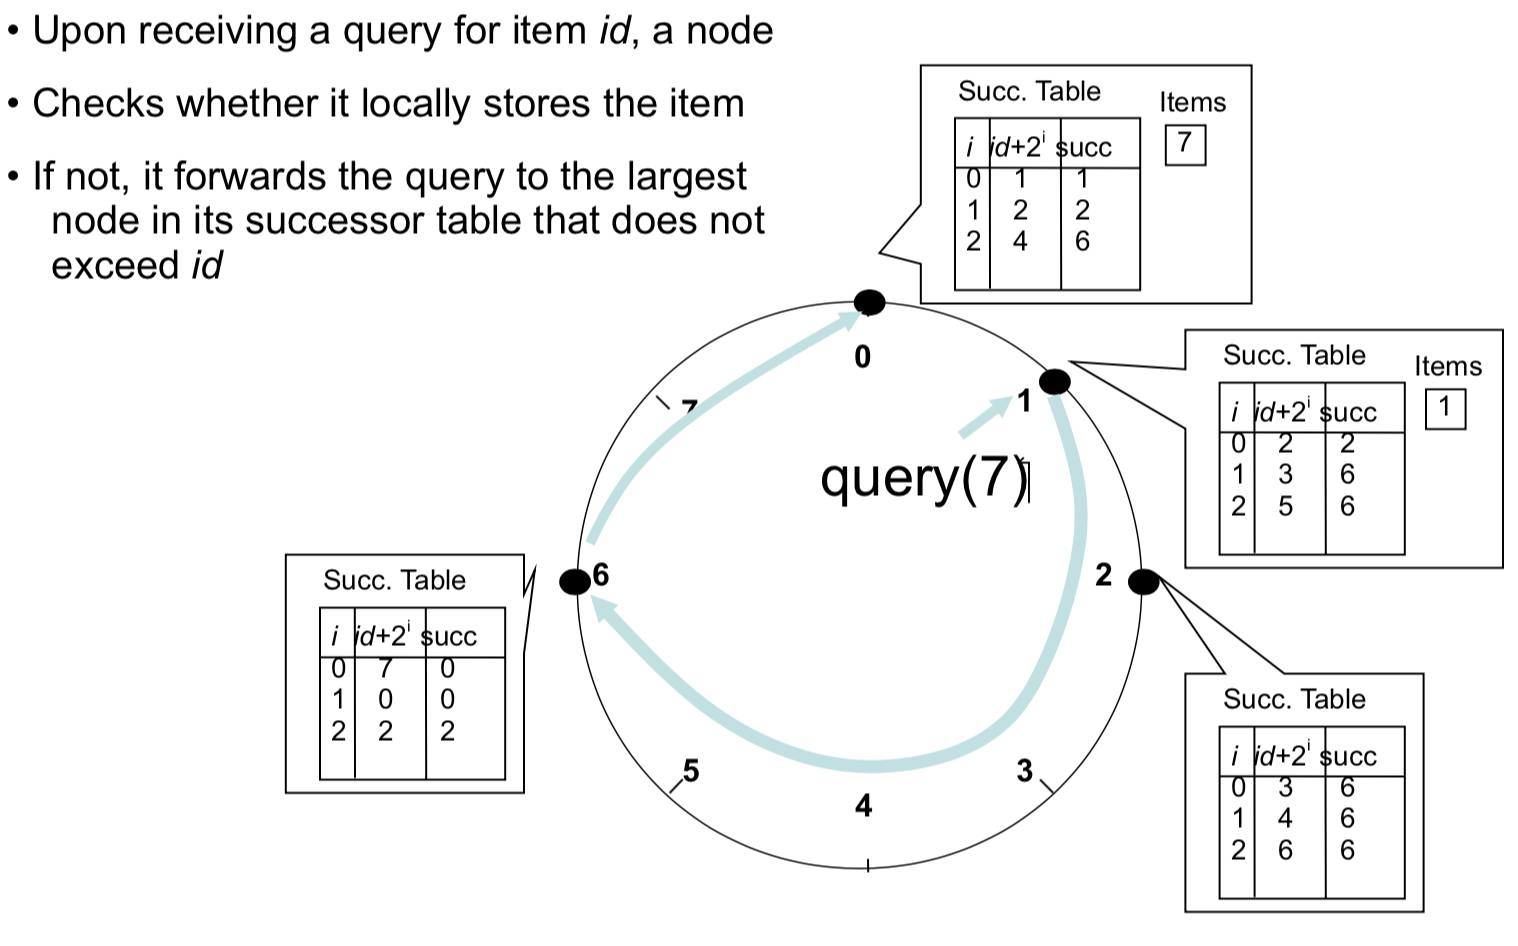
\includegraphics[width=1\textwidth]{img/chord_query.png}
  \caption{Routing after having received a query}
  \label{fig:boat1}
\end{figure}
\newpage
\section*{Mobile agents and the black hole problem}
\textbf{Definition:} Consider that we have some mobile agents that can travel across the graph and could communicate together with a whiteboard and they also have some storage, the problem is to find a malicious node (black hole) that makes disappear our mobile agents. Each agent knows the number of nodes.\\
\subsection*{Cautious walk}
We can consider our graph as a set of ports and in every port there is a traffic light. If the next port has not been controlled, the traffic light is red, going to the next node we activate it (yellow light), and when we come back from that node, that edge (and the next node) is safe (not the black hole). \\
What about if the configuration of the graph is a ring?\\
We need two agents! \\
The agents, starting from the home base, must explore using cautious walk. The agents must explore disjoint areas otherwise they could both disappear. So they finally explore step by step all the ring until one of the two agents disappear of they finish the graph and the last node that has not been marked is the black hole.
 \begin{figure}[H]
  \centering
  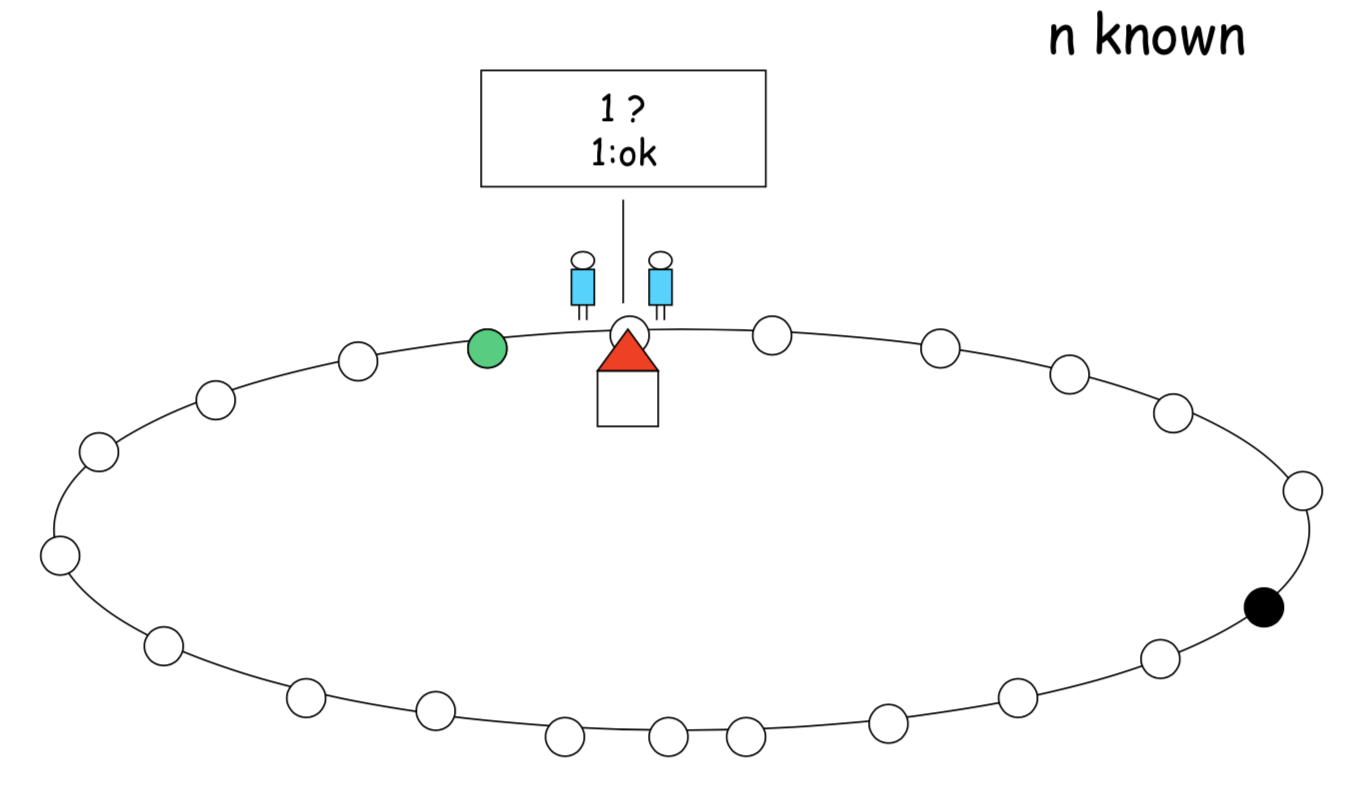
\includegraphics[width=0.5\textwidth]{img/ring1.png}
  \caption{First step of the left agent}
  \label{fig:boat1}
\end{figure} \begin{figure}[H]
  \centering
  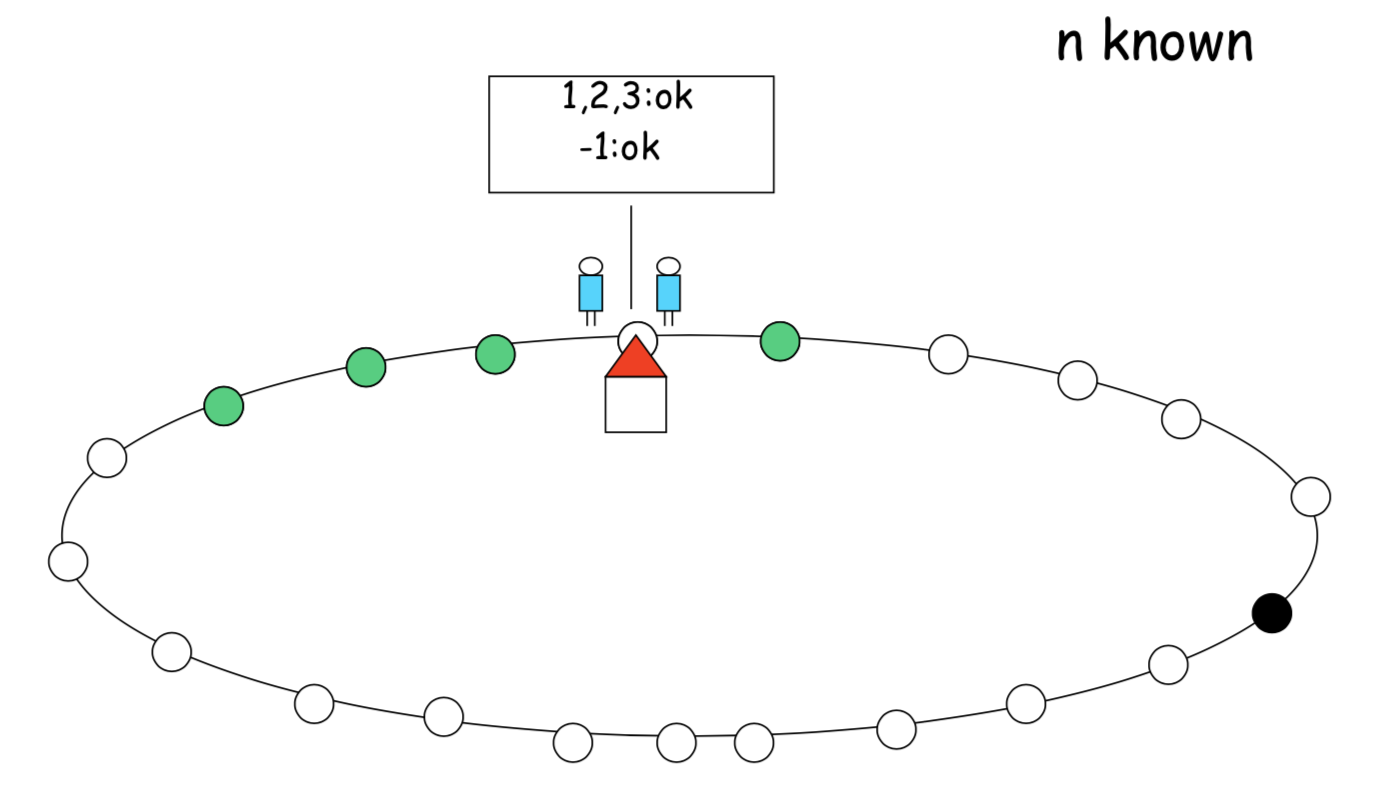
\includegraphics[width=0.5\textwidth]{img/ring2.png}
  \caption{First step of the right agent}
  \label{fig:boat1}
\end{figure} \begin{figure}[H]
  \centering
  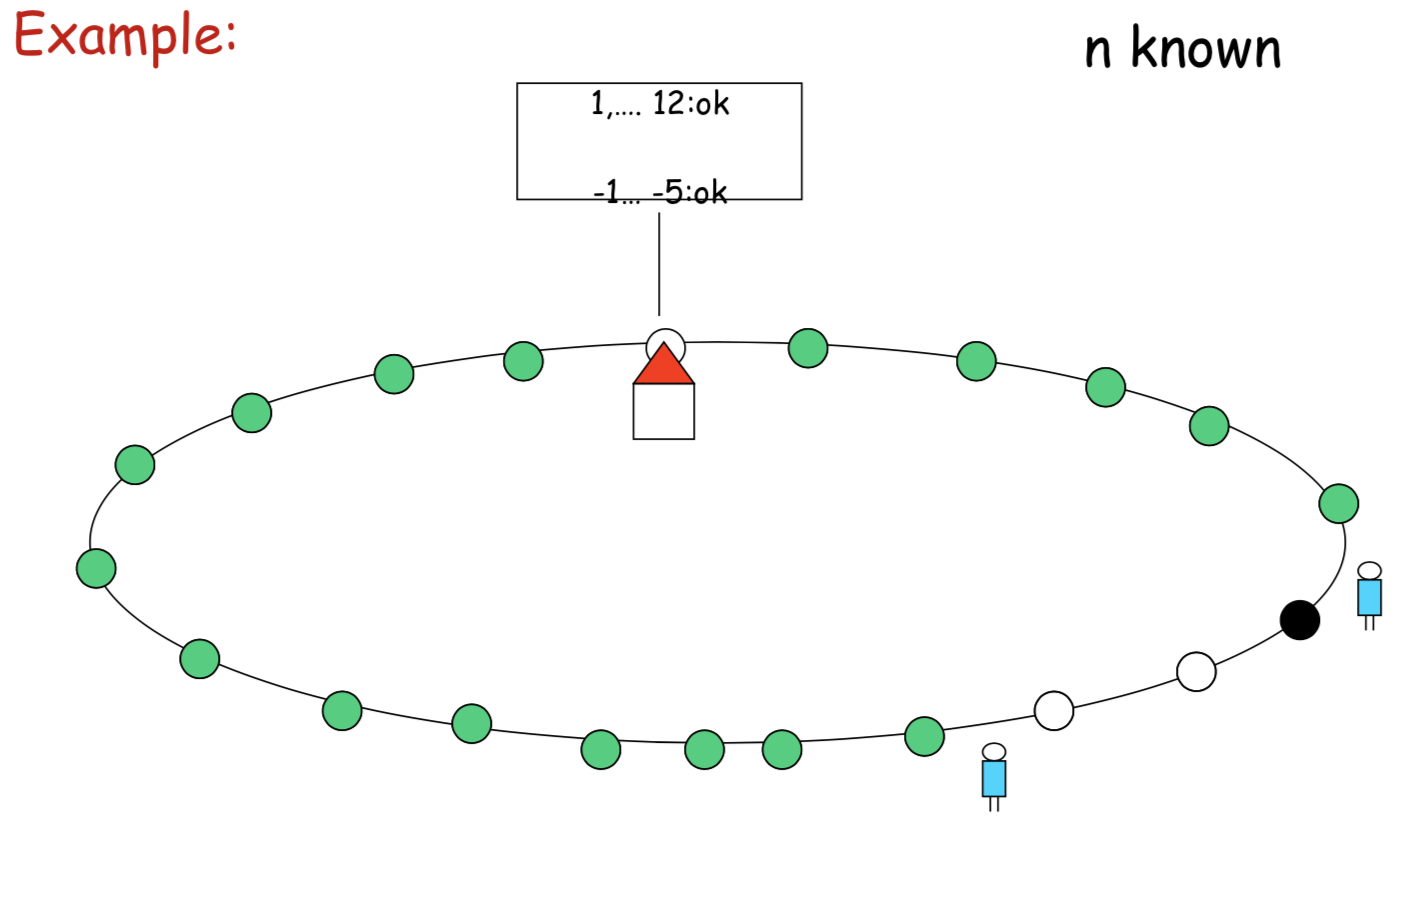
\includegraphics[width=0.5\textwidth]{img/ring3.png}
  \caption{Black hole for the right agent}
  \label{fig:boat1}
\end{figure} \begin{figure}[H]
  \centering
  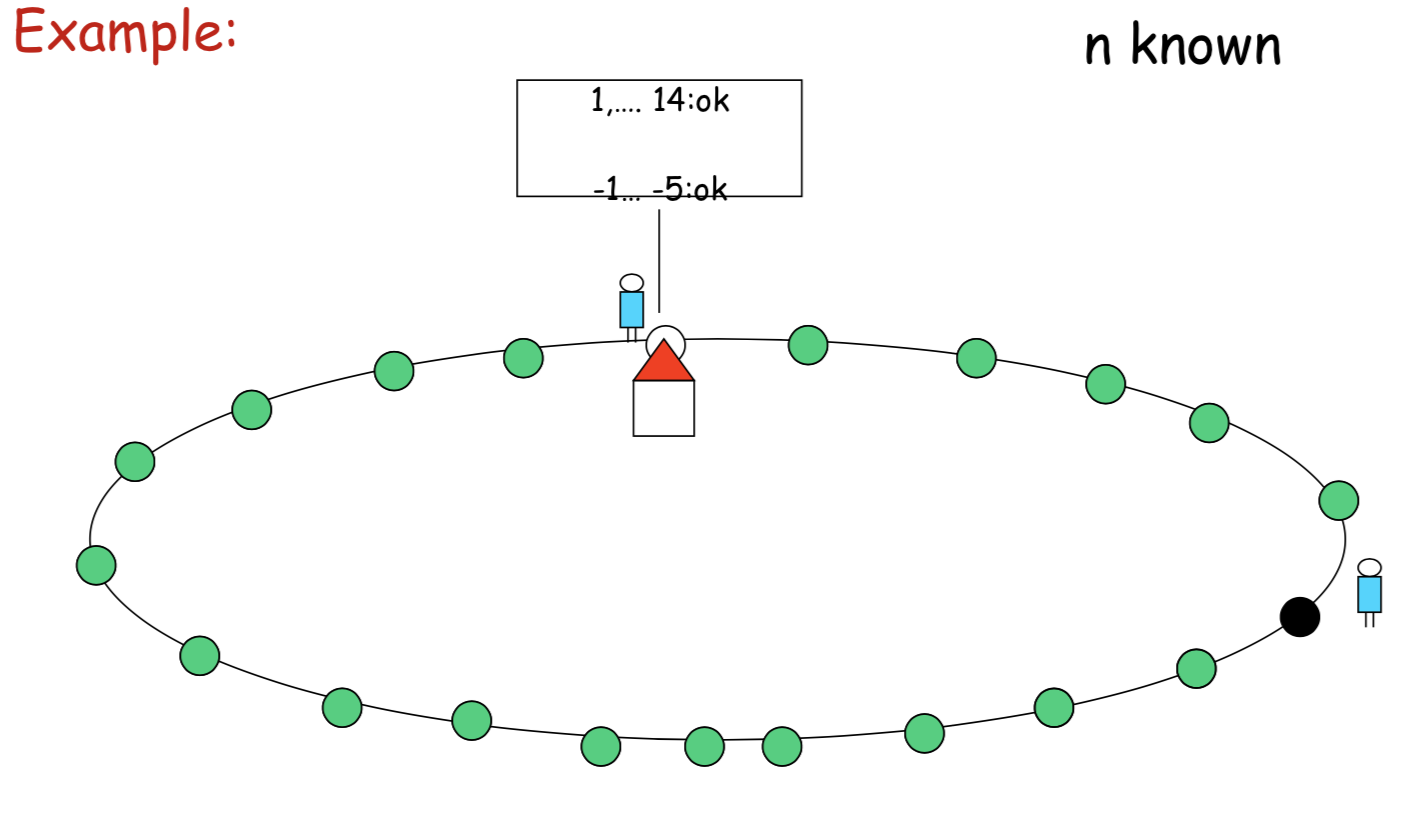
\includegraphics[width=0.5\textwidth]{img/ring4.png}
  \caption{Left agent complete the ring and knows where is the black hole (for the whiteboard)}
  \label{fig:boat1}
\end{figure}
But what if also the intruder is mobile? \\
\subsection*{The intruder capture problem}
Let's put some rules, the intruder:
\begin{itemize}
\item can moves from a node to a neighbouring one
\item can moves arbitrarily fast
\item cannot cross a node guarded by an agent
\item is invisible to the agents
\item can permanently see the position of the other agents
\end{itemize}
Initially the agents are located at the homebase and form a team while in the end the agents capture (surround) the intruder. \\
The intruder capture problem is equivalent to the decontamination problem.\\
As said initially the agents are located at the homebase and form a team. The whole network is contaminated (except the homebase). An agent cleans a node when it enters in it. At the end the whole network must be clean.\\
\textbf{Contamination rule:} a node is contaminated if it is not protected by an agent and at least one of its neighbors is contaminated (remember that the intruder is fast). 
\begin{figure}[H]
  \centering
  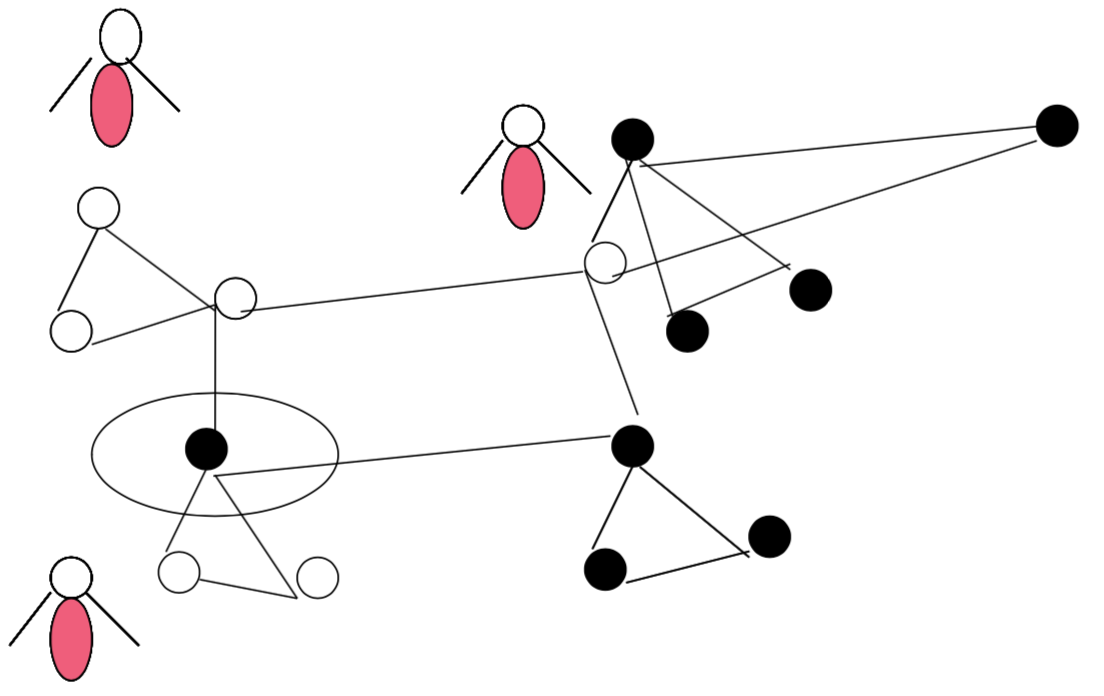
\includegraphics[width=0.5\textwidth]{img/cont.png}
  \caption{Contaminated node}
  \label{fig:boat1}
\end{figure}
\textbf{Decontamination process:} As said several times, initially the agents are located at the homebase and form a team. The whole network is contaminated (except the homebase). An agent cleans a node or an edge when it enters (or traverse the edge) in it, a node should not be recontaminated. A node becomes contaminated if it is not protected by an agent and at least one of its neighbors is contaminated.\\
\subsection*{Contiguous monotone strategies}
We consider the situration where agent move only to neighbouring nodes (contiguous) and no recontamination can occur(monotone).
\begin{figure}[H]
  \centering
  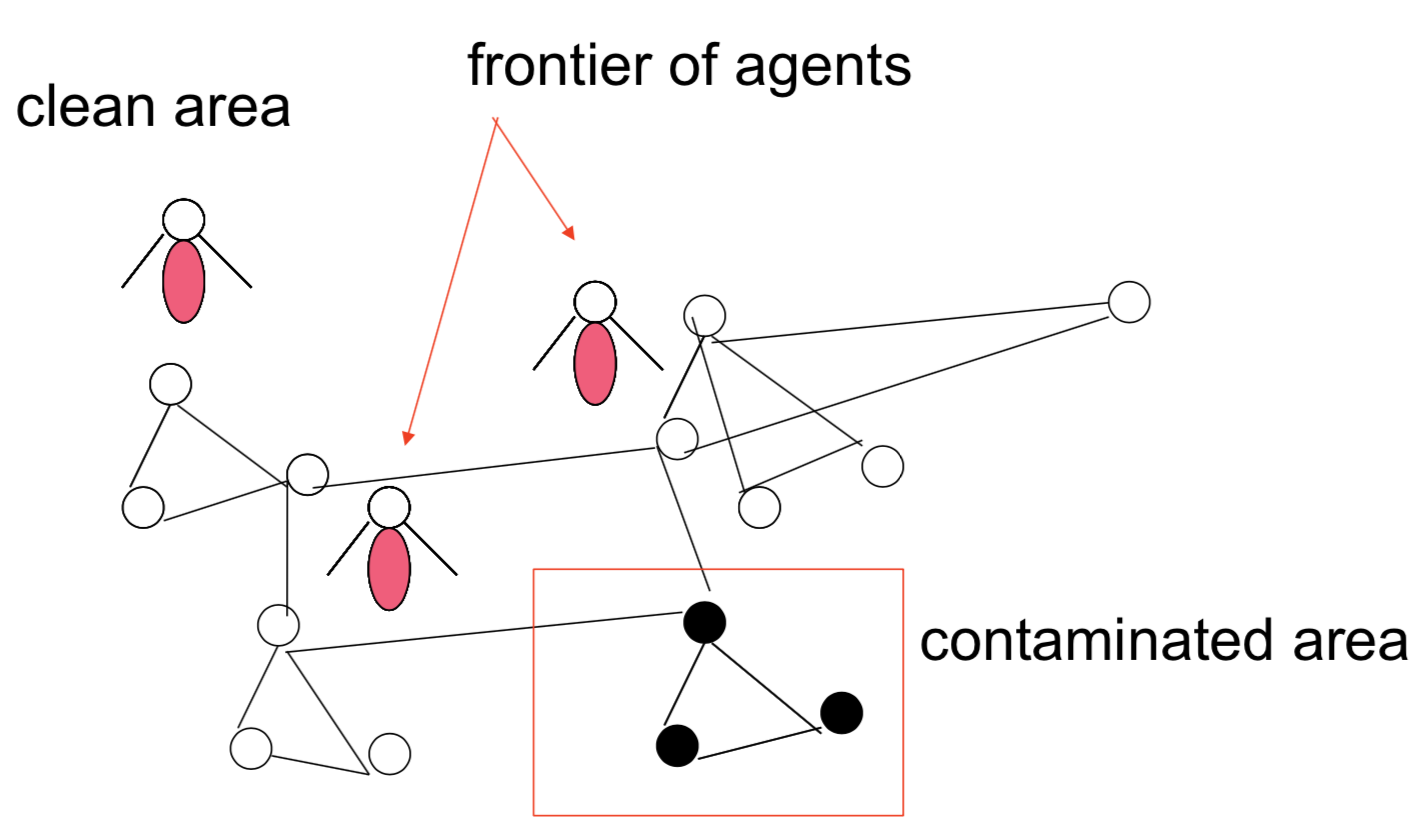
\includegraphics[width=0.5\textwidth]{img/cont_2.png}
  \caption{Contaminated node}
  \label{fig:boat1}
\end{figure}
\textbf{Complexity issues:}
\begin{itemize}
\item Number of agents
\item Number of moves
\item Time (sync or async)
\item Memory (agents, nodes(whiteboard))
\end{itemize}
Strategies are not necessarily connected and monotone (i.e. agents can jump. We have to minimize the number of searchers).\\
There are two model of visibility, one with visibility of the other neighbors (clean, contaminated, guarded) and the other in which agents have only local knowledge.
\subsubsection*{Decontaminating a mesh}
We have to be in this situation: 
\begin{itemize}
\item Asynchronous system
\item Node + agent storafe $O(\log(n))$ bits
\item Models (visibility, local)
\end{itemize}
We consider a m x n mesh topology. We have two possible strategies:
\begin{itemize}
\item With synchronizer: Searching agents do not have visibility power. The synchronizer is an agent that coordinates the moves.
\item Agents with visibility: Visibility power means agent can see their neighbouring nodes, agents can move independently, the synchronizer is not required.
\end{itemize}
The main idea behind the strategy is to: 
\begin{itemize}
\item Start from the homebase
\item Contiguously clean the contaminated network by maintaining a vertical barrier of agents (to avoid recomtamination, works asynchronously)
\item Move one column at the time
\end{itemize}
\begin{figure}[H]
  \centering
  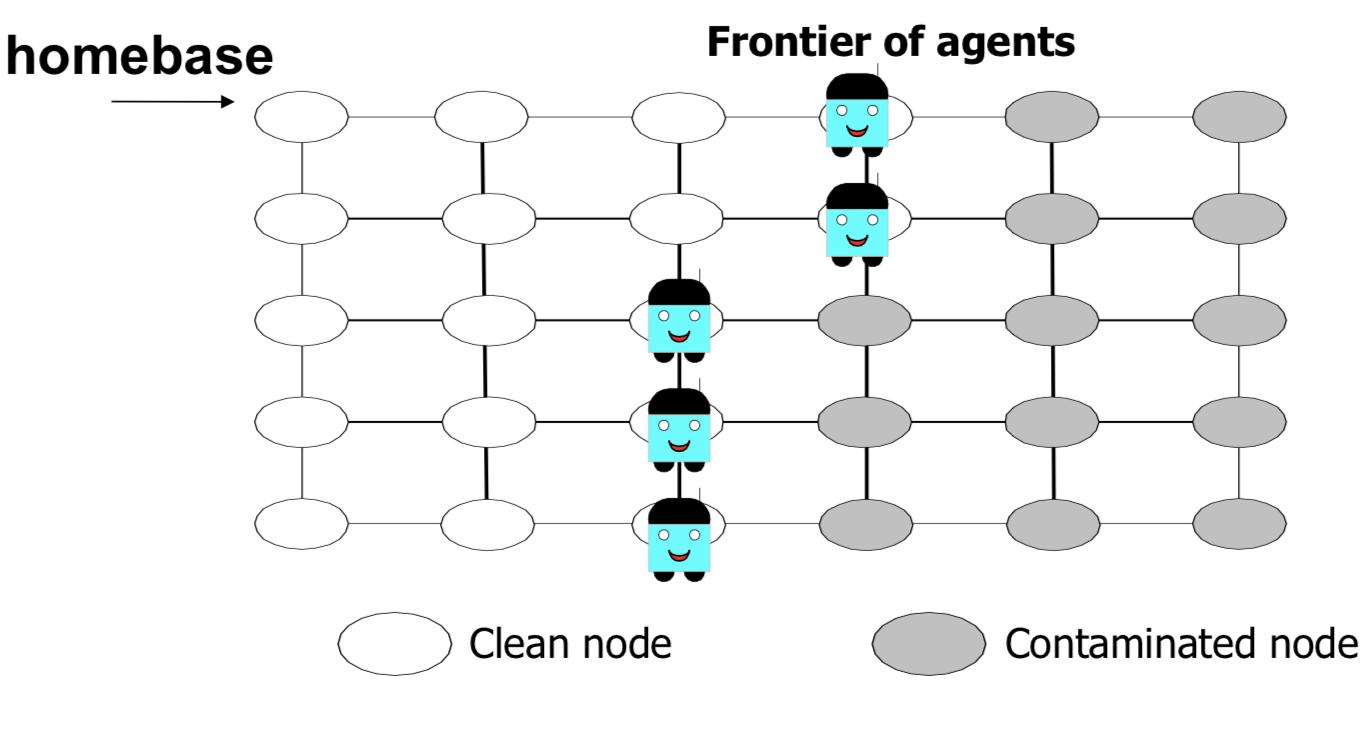
\includegraphics[width=0.5\textwidth]{img/cont_front.png}
  \caption{Contaminated node}
  \label{fig:boat1}
\end{figure}
We can perform the search of a node or of an edge moving the barrier. (see slides)

\end{document}
